\documentclass[a4paper,11pt]{scrartcl}
\usepackage[top=2cm,bottom=2cm,left=2.5cm,right=2.5cm]{geometry} % Seitenränder einstellen
\usepackage[english]{babel} % Worttrennung nach der neuen Rechtschreibung und deutsche Bezeichnungen
\usepackage[utf8]{inputenc} % Umlaute im Text
%\usepackage[scaled]{helvet} % Schriftart Helvetica
%\renewcommand*\familydefault{\sfdefault} %% Only if the base font of the document is to be sans serif
\usepackage[T1]{fontenc} % Trennung von Umlauten
\usepackage[dvipsnames]{xcolor} % Farbe in Dokument
\definecolor{tumblau}{rgb}{0,0.40234375,0.7734375} % eigene Farbe definieren
\parindent 0pt % kein Einrücken bei neuem Absatz
\usepackage{amsmath} % zusätzliche mathematische Umgebungen
\usepackage{amssymb} % zusätzliche mathematische Symbole
%\usepackage{bbold} % zusätzliche mathematische Symbole
\usepackage{units} % schöne Einheiten und Brüche
\usepackage[square]{natbib} % wissenschaftliches Literaturverzeichnis
%\usepackage[printonlyused]{acronym} % Abkürzungsverzeichnis
\usepackage{icomma} % kein Leerzeichen bei 1,23 in Mathe-Umgebung
\usepackage{wrapfig} % von Schrift umflossene Bilder und Tabellen
\usepackage{picinpar} % Objekt in Fließtext platzieren (ähnlich zu wrapfig)
\usepackage{scrhack} % verbessert andere Pakete, bessere Interaktion mit KOMA-Skript
\usepackage{float} % bessere Anpassung von Fließobjekten
\usepackage{pgf} % Makro zur Erstellung von Graphiken
\usepackage{tikz} % Benutzeroberfläche für pgf
\usepackage[
margin=10pt,
font=small,
labelfont=bf,
labelsep=endash,
format=plain
]{caption} % Einstellungen für Tabellen und Bildunterschriften
\usepackage{subcaption} % Unterschriften für mehrere Bilder
\usepackage{enumitem} % no indentation at description environment
\usepackage[onehalfspacing]{setspace} % Änderung des Zeilenabstandes (hier: 1,5-fach)
\usepackage{booktabs} % Einstellungen für schönere Tabellen
\usepackage{graphicx} % Einfügen von Grafiken -> wird in master-file geladen
\usepackage{url} % URL's (z.B. in Literatur) schöner formatieren
\usepackage[pdftex]{hyperref} % Verweise innerhalb und nach außerhalb des PDF; hyperref immer als letztes Paket einbinden
\hypersetup{
pdftitle = {},
pdfauthor = {},
pdfsubject = {},
pdfproducer = {LaTeX},
pdfkeywords = {},
colorlinks,
linkcolor = black,
citecolor = black,
filecolor = black,
urlcolor = blue
} % Einstellungen Dokumenteigenschaften und Farbe der Verweise
%\usepackage{pythonhighlight} % python highlighting

% define bordermatrix with brackets
\makeatletter
\def\bbordermatrix#1{\begingroup \m@th
  \@tempdima 4.75\p@
  \setbox\z@\vbox{%
    \def\cr{\crcr\noalign{\kern2\p@\global\let\cr\endline}}%
    \ialign{$##$\hfil\kern2\p@\kern\@tempdima&\thinspace\hfil$##$\hfil
      &&\quad\hfil$##$\hfil\crcr
      \omit\strut\hfil\crcr\noalign{\kern-\baselineskip}%
      #1\crcr\omit\strut\cr}}%
  \setbox\tw@\vbox{\unvcopy\z@\global\setbox\@ne\lastbox}%
  \setbox\tw@\hbox{\unhbox\@ne\unskip\global\setbox\@ne\lastbox}%
  \setbox\tw@\hbox{$\kern\wd\@ne\kern-\@tempdima\left[\kern-\wd\@ne
    \global\setbox\@ne\vbox{\box\@ne\kern2\p@}%
    \vcenter{\kern-\ht\@ne\unvbox\z@\kern-\baselineskip}\,\right]$}%
  \null\;\vbox{\kern\ht\@ne\box\tw@}\endgroup}
\makeatother



\title{\vspace{-1cm}Object Recognition and Image Understanding}
\subtitle{Exercise 6: Project Proposal} \date{\today}

\begin{document}
\maketitle

\section*{Team}
Marvin Klaus, Daniela Schacherer. We plan to work as a team, however, as we are testing two different approaches each person will have the main responsibility for one of them. We marked responsibilites when describing the approaches.

\section*{Problem Definition}
Nowadays, autonomous driving is one of the most growing research fields. In this context visual detection and recognition of traffic signs is of particular importance. Our project aims at the exploration and comparison of two different approaches towards the detection of road signs in color images. Detection means that we will locate the traffic signs in the images, however, do not yet classify them.

\section*{Dataset}
There are various freely available datasets containing street scenes. We finally decided to use a set of images provided by the University of Bochum as part of a traffic sign detection competition in 2013: \url{http://benchmark.ini.rub.de/?section=gtsdb&subsection=dataset}. The data consist of a training set (900 images provided in PPM format) as well as a test data set. 
Figure \textit{1} shows an example. 

% include a picture
	\begin{figure}[htbp] 
		\centering	
		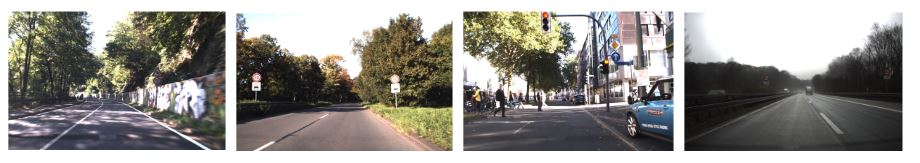
\includegraphics[width=\linewidth]{./example}
		\label{fig:ex}
		\caption{Example image from the dataset}
	\end{figure}


\section*{Approach}
In this project we will go through two different approaches and eventually compare the results of both. \\
In the first approach (main responsiblity: Daniela) we will use RGB color segmentation followed by shape matching. Therefore we first apply filters on each color channel to select those regions in the image (ROIs) where the pixel values fall within the range of our target object - which might be a red stop sign or a blue sign for the prescribed direction of travel. It might be challenging to find the appropriate thresholds for each color channel such that no traffic signs are missed. In a second step a shape-based matching approach (like e.g. Hough transform) will be used to further observe the ROIs and decide whether there is a road sign or not. If we consider it necessary in the course of the project we will apply preprocessing techniques for example to reduce the amount of noise in the images. \\
We will compare the results and the performance of this first approach 
with the second one (main responsibility: Marvin). In this one we create a R-CNN to correctly locate traffic signs in the image via a bounding box. In our 
first design each feature extraction stage of the network consists of a 
convolutional layer, a non-linear transformation layer and a spatial 
pooling layer. In accordance with the standard, the last layers will be fully-connected. To enter pictures into the network, every image needs to be the same 
size. So depending on the dataset, we need to warp the images before 
using them.


\section*{Evaluation and expected results}
For the first approach we will measure the accuracy as the fraction of traffic signs which our algorithm detects in all images of the test set. We expect good results (about at least 70\% of traffic signs detected), however the second approach may outperform this. \\
For the R-CNN we evaluate the accuracy of our network over 
time for the training and the separate test set. Since we compare the 
computed bounding box with the given ones, the exact pixels of the boxes 
are probably hard to predict, a little deviation is to be expected. At 
the moment we can't tell how good our network will work, but we aim at 
an accuracy beyond 90\% of the boxes.
On the topic of performance it is hard to tell how fast our network 
should be. Since this is a field of autonomous driving we want to get a 
result in a part of a second so that it is a realistic traffic sign 
recognition network. To use some network like this in practice, classification would be needed on top and both together still should give a reliable 
result in less than a second.


\end{document}